\section{Обзор}

Под \textit{контекстно-свободной аппроксимацией} подразумевается грамматика, описывающая контекстно-свободный язык, который содержит в качестве подмножества возможные значения динамически формируемого выражения. 
Идея использования такой аппроксимации была заимствована из существующих работ в области анализа динамически формируемого кода, краткий обзор которых будет приведен в данной секции. 
Алгоритм синтаксического анализа регулярной аппроксимации на основе GLL был адаптирован нами для работы c графовым представлением КС-грамматик. 
В качестве такого представления мы использовали Grammar Flow Graph (GFG,~\cite{kovalev-spbu-gfg}). Описания оригинального алгоритма и GFG также включены в обзор. 

\subsection{Подходы к анализу динамически формируемых выражений}

Существует два основных подхода, позволяющих проводить различные виды анализа динамически формируемого кода. 
Один из них основан на проверке включения языка, аппроксимирующего множество значений динамически формируемого выражения, в эталонный контекстно-свободный язык, заданный пользователем. 
Данный подход был реализован в инструментах Java String Analyzer (JSA,~\cite{kovalev-spbu-jsa}) и PHP String Analyzer (PHPSA,~\cite{kovalev-spbu-phpsa}).
Получение аппроксимации в них реализовано следующим образом --- из исходного кода программы извлекается набор dataflow-уравнений, описывающих значения строковых переменных, которые участвуют в генерации выражения. 
Эти уравнения затем интерпретируются как контекстно-свободная грамматика, описывающая аппроксимирующий язык. 
PHPSA работает непосредственно с такой грамматикой, используя эвристики (т.к. в общем случае задача о включении КС-языков неразрешима~\cite{kovalev-spbu-lang_inclusion}); в JSA контекстно-свободный язык дополнительно аппроксимируется регулярным.

Другой подход заключается в проведении синтаксического анализа аппроксимации множества значений выражения. 
Такое решение позволяет не просто ответить на вопрос о включении языков, но и реализовать дополнительную функциональность, такую как вычисление семантики или рефакторинг. 
К методам, основанным на данном подходе, можно отнести алгоритмы синтаксического анализа регулярной аппроксимации на базе семейства GLR~\cite{kovalev-spbu-alvor, kovalev-spbu-rnglr_reg} и GLL-алгоритмов~\cite{kovalev-spbu-gll_reg}, а также алгоритм абстрактного синтаксического анализа~\cite{kovalev-spbu-a_lr}, позволяющий совместить синтаксический анализ с решением dataflow-уравнений, получаемых при помощи PHPSA.

\subsection{Синтаксический анализ регулярной аппроксимации на основе GLL}

Generalized LL (GLL)~\cite{kovalev-spbu-gll} --- алгоритм синтаксического анализа, позволяющий, в отличие от классических LL-анализаторов, работать с произвольными контекстно-свободными грамматиками. 
При этом, GLL сохраняет такие важные свойства алгоритмов нисходящего разбора, как интуитивная связь с грамматикой и простота отладки и диагностики ошибок.

Основной идеей GLL является использование дескрипторов, позволяющих полностью описывать состояние анализатора в текущий момент времени.

\begin{definition}
    Дескриптор --- это четверка (L, u, i, N), где
    \begin{itemize}
        \setlength\itemsep{0em}
        \item L --- текущая позиция в грамматике вида $A \rightarrow \alpha \cdot \beta$
        \item u --- текущая вершина Graph Structured Stack (GSS,~\cite{kovalev-spbu-tomita})
        \item i --- позиция во входном потоке
        \item N --- построенный на данный момент узел дерева вывода  
    \end{itemize}
\end{definition}  

В процессе работы поддерживается глобальная очередь дескрипторов. В начале каждого шага исполнения алгоритм берет следующий в очереди дескриптор и производит действия в зависимости от позиции в грамматике и текущего входного символа. 
Для обработки неоднозначностей в грамматике алгоритм добавляет дескрипторы для каждого возможного пути анализа в конец очереди. Результат работы алгоритма --- множество деревьев разбора строки (лес разбора) --- представляется в виде Shared Packed Parse Forest (SPPF)~\cite{kovalev-spbu-sppf}.

В рамках магистерской диссертации~\cite{kovalev-spbu-gll_reg} на базе GLL был разработан алгоритм для синтаксического анализа регулярной аппроксимации множества значений динамически формируемого выражения. 
Под регулярной аппроксимацией здесь понимается детерминированный конечный автомат над алфавитом токенов (рис.~\ref{fig:app_r}). Оригинальный GLL-алгоритм был модифицирован для работы с нелинейным входом. 
Дескрипторы нового алгоритма хранят номер вершины входного графа вместо позиции в линейном потоке. Также, на шаге исполнения просматривается не единственный входной символ, а все ребра, исходящие из текущей вершины. Псевдокод данного алгоритма можно увидеть в приложении \ref{gll_code}. Основная логика работы представлена в функциях \textbf{dispatcher} (извлечение дескрипторов из очереди) и \textbf{processing} (анализ исходящих из текущей вершины ребер).

\subsection{Grammar Flow Graph}

Grammar Flow Graph (GFG,~\cite{kovalev-spbu-gfg}) --- связный помеченный граф, узлы которого соответствуют позициям в грамматике ($A \rightarrow \alpha \cdot \beta$). Различают следующие типы узлов ($X$ --- нетерминальный символ, $t$ --- терминальный):
\begin{itemize}
    \setlength\itemsep{-0.2em}
    \item[--] $A \rightarrow \alpha \cdot X \beta   $ --- call
    \item[--] $A \rightarrow \alpha X \cdot \beta$ --- return
    \item[--] $A \rightarrow \cdot \alpha$ --- entry
    \item[--] $A \rightarrow \alpha \cdot$ --- exit
    \item[--] $A \rightarrow \alpha \cdot t \beta$ --- scan
\end{itemize}
Для обозначения подграфа, представляющего продукции, имеющие в левой части нетерминал $A$, дополнительно используются узлы с метками $.A$ (start-узел) и $A.$ (end-узел). Подробное описание GFG можно найти в оригинальной статье.

Приведем определение выводимости строки в грамматике в терминах GFG. Для этого нам потребуется также определить понятие сбалансированного пути.

\begin{definition}
    Сбалансированным путем в GFG называется путь, подпоследовательность call- и return-узлов которого сбалансирована. 
\end{definition}

\begin{definition}
    Строка $w$ выводима в грамматике, если в GFG существует сбалансированный путь из узла $.S$ в узел $S.$ (здесь S --- стартовый нетерминал грамматики), и $w$ может быть получена конкатенацией меток на ребрах, содержащихся в данном пути. 
\end{definition}

\begin{figure}[!h]
	\centering
	\begin{subfigure}[h!]{0.33\textwidth}
		\centering
		\begin{minipage}{5cm}
			\begin{Verbatim}[commandchars=\\\{\}]
expr = \textcolor{red}{"a"}
while (...)
  expr = \textcolor{red}{"("} + expr + \textcolor{red}{")"}
print expr
			\end{Verbatim}
		\end{minipage}
		\caption{Исходный код}
		\label{fig:code}
	\end{subfigure}
	\hfill
	\begin{subfigure}[h!]{0.3\textwidth}
		\centering
		$
		\begin{array}{crcl}
			&s' &::=& s \\
			&s & ::= & \mbox{\texttt{LBR }} s \mbox{\texttt{ RBR}}\\
			&s & ::= & \mbox{\texttt{A}}
		\end{array}
		$
		\caption{КС-аппроксимация}
		\label{fig:app_cf}
	\end{subfigure}
	\hfill
	\begin{subfigure}[h!]{0.3\textwidth}
		\centering
		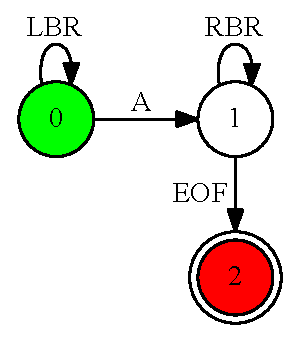
\includegraphics[width=2.5cm]{pictures/kovalev-spbu-reg_app}
		\caption{Регулярная}
		\label{fig:app_r}
	\end{subfigure}
	\caption{Исходный код и примеры аппроксимаций}
	\label{example}
\end{figure}

\begin{figure}[h]
    \centering
    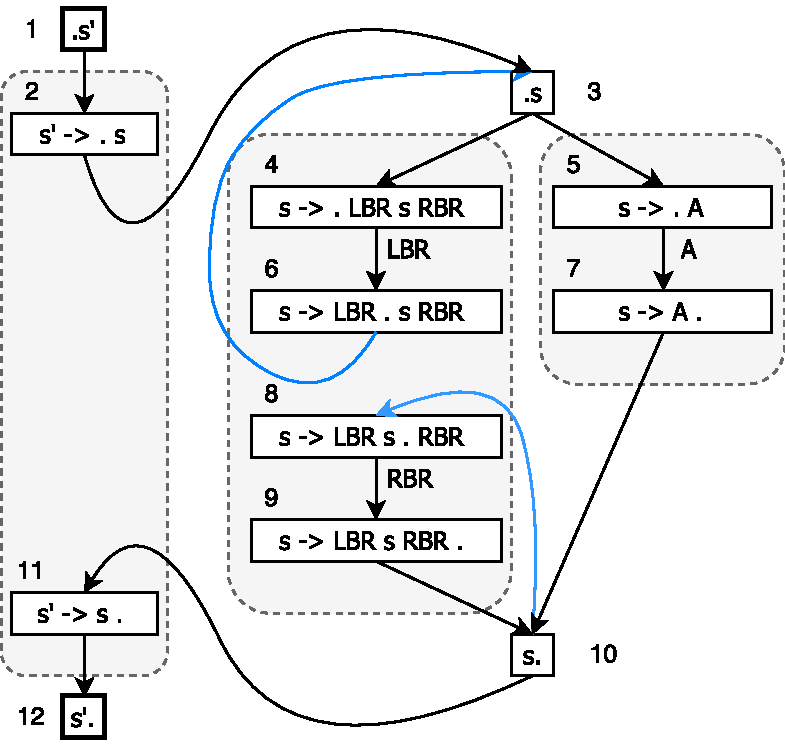
\includegraphics[width=0.5\textwidth]{pictures/kovalev-spbu-gfg_enum}
    \caption{GFG для грамматики \ref{fig:app_cf}}
    \label{fig:gfg}
\end{figure}
